\section{Analysis}
\label{sec:Analysis}

At first the detector has to be calibrated, after which different gamma spectra are measured. The analysis of this data is following.
Before that the background has to be measured, which is shown in \autoref{fig:underground}. In this the counts per second in the different channels are shown.
It is calculated by dividing the absolute counts by the time in seconds for which it was measured, which was 21 hours and 11 minutes.
\begin{figure}[htbp]
    \centering
    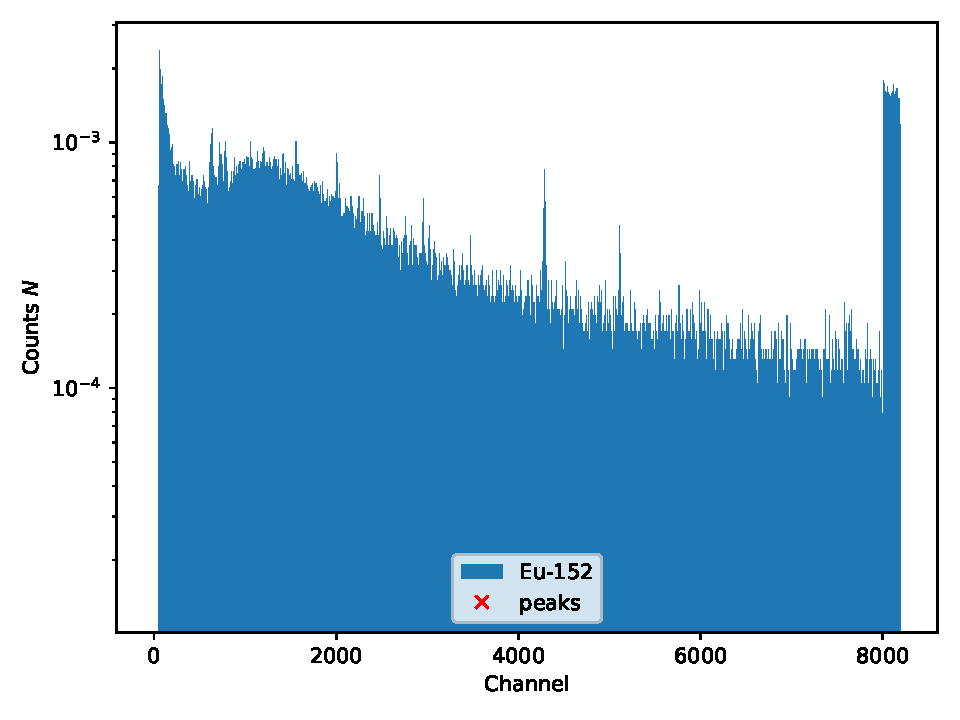
\includegraphics[width=0.8\textwidth]{content/plots/Underground.pdf}
    \caption{Measured background spectrum, which is subtracted from all following spectra.}
    \label{fig:underground}
\end{figure}

This result is used by subtracting it from all following measured spectra.
By this the background is removed from the real measurements.

\subsection{Detector calibration with \texorpdfstring{\ce{^{152}Eu}}{152Eu}}

To begin, the channels of the multichannel analyser have to be calibrated.
To do that the measurements of \ce{^{152}Eu} are depicted in \autoref{fig:eu_calibration}, in which multiple peaks are visible.
The peaks are found with scipy and compared with the known gamma spectrum shown in \autoref{tab:Euspec}.
The data above channel 8000 is not used, because it is only overflow data from all data above the measuring window.

\begin{figure}[htbp]
    \centering
    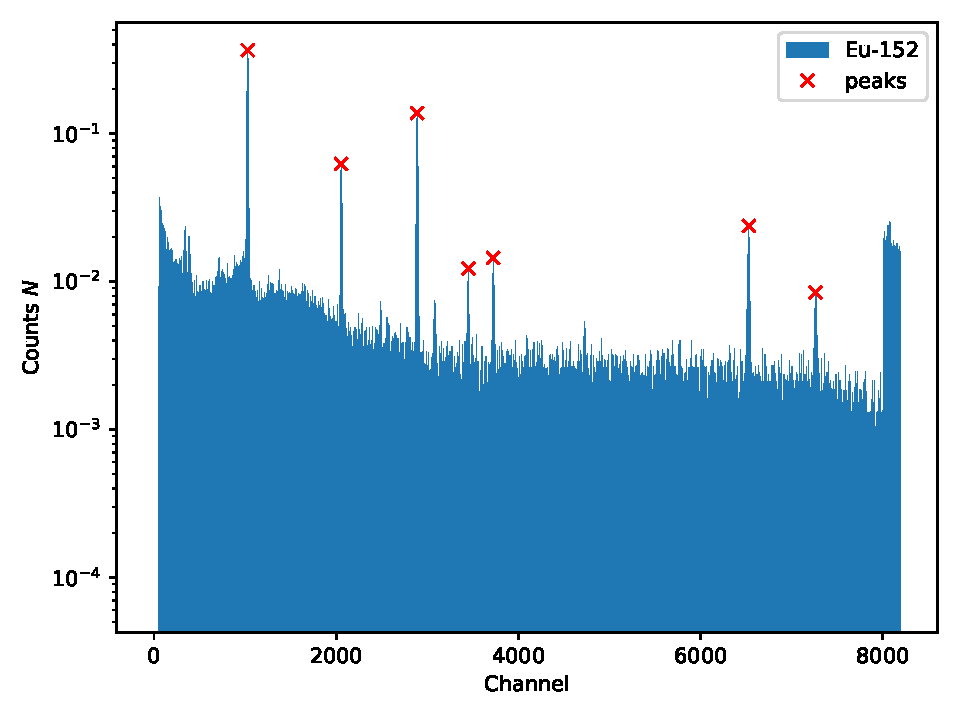
\includegraphics[width=0.8\textwidth]{content/plots/eu_calibration.pdf}
    \caption{Measured spectrum of \ce{^{152}Eu} with the peaks used for the calibration.}
    \label{fig:eu_calibration}
\end{figure}
The channels and the energies are plotted in \autoref{fig:eu_linear_fit}. With this data a linear regression in the form
\begin{equation}
    \label{eqn:lin}
    E = m \cdot K + b
\end{equation}
with the energy $E$ and the channel $K$
is done, which is also seen in the plot.
This regression gives the parameters
\begin{align}
    m &= \SI{0.11950 \pm 0.00005}{keV}\text{/channel} \\
    b &= \SI{-0.98 \pm 0.23}{keV} \ .
\end{align}

\begin{figure}[htbp]
    \centering
    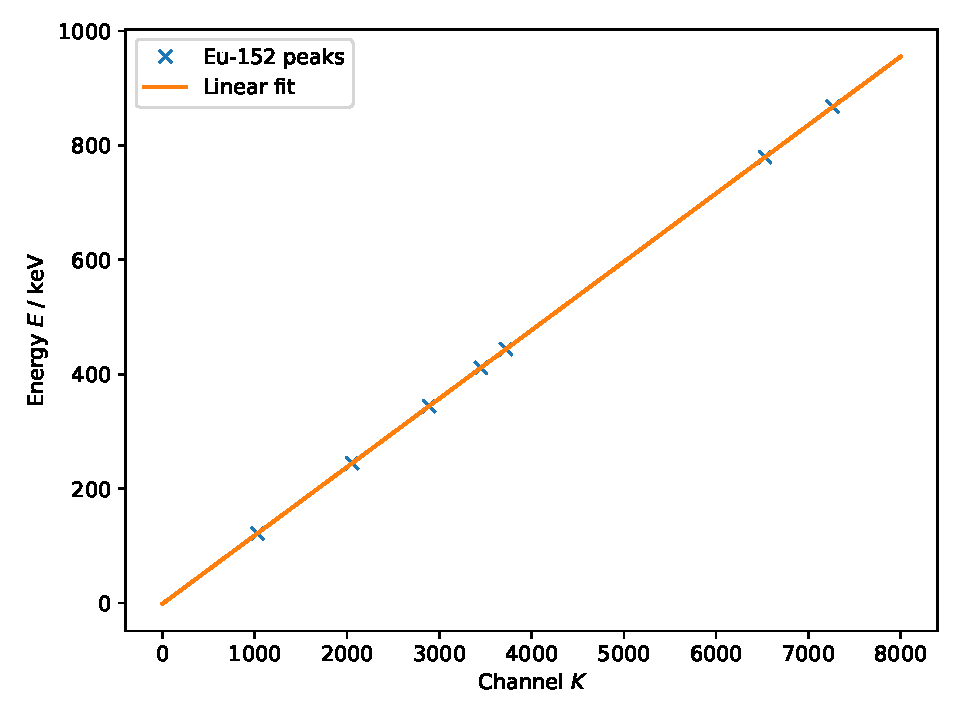
\includegraphics[width=0.8\textwidth]{content/plots/eu_linear_fit.pdf}
    \caption{Literature energies of the \ce{^{152}Eu} lines against the measured channels with a linear fit.}
    \label{fig:eu_linear_fit}
\end{figure}


\begin{table}[H]
	\centering
	\caption{Energies $E_\gamma$ and emission probabilities $W$ of the used \ce{^{152}Eu} gamma lines~\cite{eu152}.}
	\label{tab:Euspec}
	\begin{tabular}{c | c}
		\toprule
		$E_\gamma$ / keV & $W$ / \%\\
		\midrule
		121.78 & 28.580  \, \clap{$\pm$} \,  0.090 \\
		 244.70 & 7.580  \, \clap{$\pm$} \,  0.030 \\
		 344.28 & 26.50  \, \clap{$\pm$} \,  0.60 \\
		 411.12 & 2.234  \, \clap{$\pm$} \,  0.025 \\
		 443.96 & 3.148  \, \clap{$\pm$} \,  0.020 \\
		 778.90 & 12.94  \, \clap{$\pm$} \,  0.15 \\
		 867.37 & 4.245  \, \clap{$\pm$} \,  0.021 \\
		 \bottomrule
	\end{tabular}
\end{table}


\subsubsection*{Activity determination}

For the full energy detection probability the current activity is necessary.
It is calculated through
\begin{equation}
    A = A_0 \cdot \exp(-\ln(2)t / T_{1/2}) \ .
\end{equation}
Where $A_0$ is the activity at the production date with $A_0 = \SI{4130 \pm 60}{Bq}$, $T_{1/2}$ the half-life with $T_{1/2} = \SI{13.537}{a}$ and $t$ the time since the production in seconds, which is $t = \SI{824428800}{s}$.
This results in the current activity $A = \SI{1084 \pm 16}{Bq}$.

\subsubsection*{Line content}

The line content $N$ is the number of counts per second in a peak.
To get it, a gaussian function with a constant is fitted to every peak in a range of 40 channels around the peak.
The fit function is
\begin{equation}
    f(K) = h \cdot \exp\left(-\frac{(K-\mu)^2}{2\sigma^2}\right) + c \ .
    \label{eqn:gauss}
\end{equation}
Where $h$ is the height of the peak, $\mu$ the position, $\sigma$ the width and $c$ the background under the peak.
An example of this fit is shown in \autoref{fig:eu_gauss_fit} for the line at $\SI{344.3}{keV}$.
The line content is then the area under the gaussian function, which is
\begin{equation}
    N = \sqrt{2\pi} \cdot h \cdot \sigma \ .
\end{equation}
The results for all lines are listed in \autoref{tab:eu_Q}.


\begin{figure}[htbp]
    \centering
    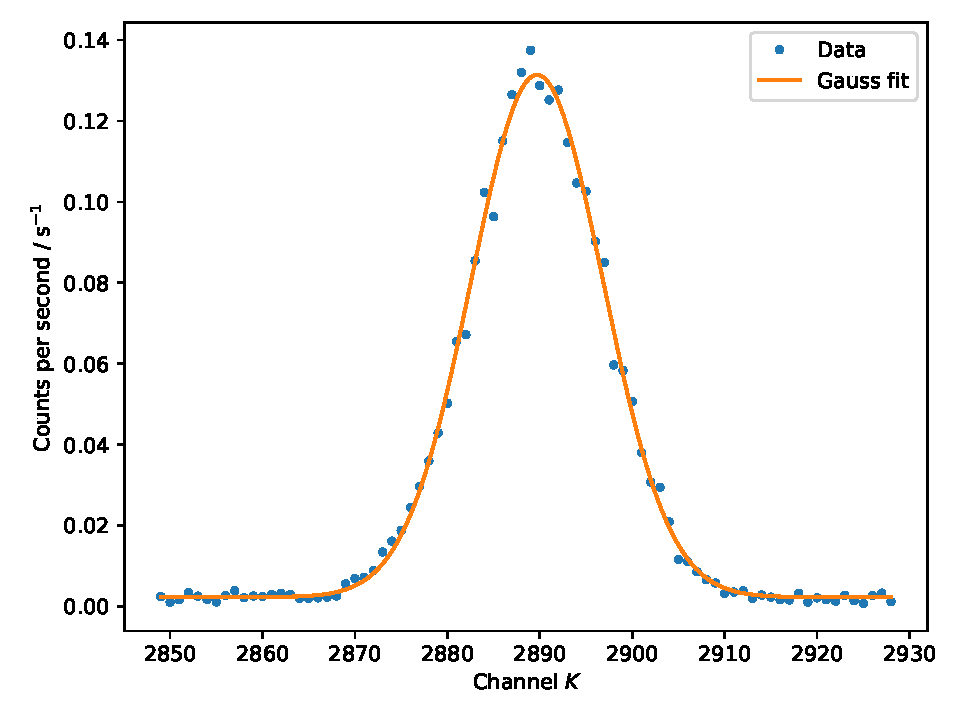
\includegraphics[width=0.8\textwidth]{content/plots/eu_gauss_fit.pdf}
    \caption{Gaussian fit of the $\SI{344.3}{keV}$ line of \ce{^{152}Eu} as an example for the determination of the line content.}
    \label{fig:eu_gauss_fit}
\end{figure}

\subsubsection*{Full energy detection probability}

The full energy detection probability is given by
\begin{equation}
    \label{eqn:Q}
    Q = N / (A\cdot W\cdot \Omega/(4\pi)) \ .
\end{equation}
Here $N$ is the measured counts per second, $W$ the emission probability of the line and $\frac{\Omega}{4\pi}$ the solid angle, which is given by
\begin{equation}
    \frac{\Omega}{4\pi} = \frac{1}{2}\left(1-\frac{a}{\sqrt{a^2+r^2}}\right) \ .
\end{equation}
Where $a = \SI{7.9}{cm}-\SI{4.675}{cm}+\SI{1.5}{cm}$ is the distance between detector and source and $r$ is the radius of the detector with $\SI{2.25}{cm}$.
The distance $a$ is calculated by the distance from the source $\SI{7.9}{cm}$ minus the distance the holder of the source is reaching back in the direction of the detector,
which is here $\SI{4.675}{cm}$. Additionally $\SI{1.5}{cm}$ from the aluminium cap is added.
With these numbers the solid angle is calculated to $\frac{\Omega}{4\pi} = \num{0.0486}$.
\\
The emission probabilities $W$ are given in \autoref{tab:Euspec} and the line contents $N$ are the ones from the gaussian fits.
The calculated values of $Q$ for every line are listed in \autoref{tab:eu_Q} and plotted in \autoref{fig:eu_efficiency}.
To describe the energy dependence of $Q$, a power function
\begin{equation}
    Q(E) = q_a \cdot E^{q_b}
\end{equation}
is fitted to the data.
Only the lines with $E > \SI{150}{keV}$ are used for the fit, because at lower energies the gamma rays are absorbed in the aluminium cap and the dead layer of the detector,
so $Q$ does not follow the power function there.
The fit gives the parameters
\begin{align}
    q_a &= \num{127 \pm 28} \\
    q_b &= \num{-1.14 \pm 0.04} \ .
\end{align}
This function $Q(E)$ is used in the following sections to determine the activities of the other sources.



\begin{figure}[htbp]
    \centering
    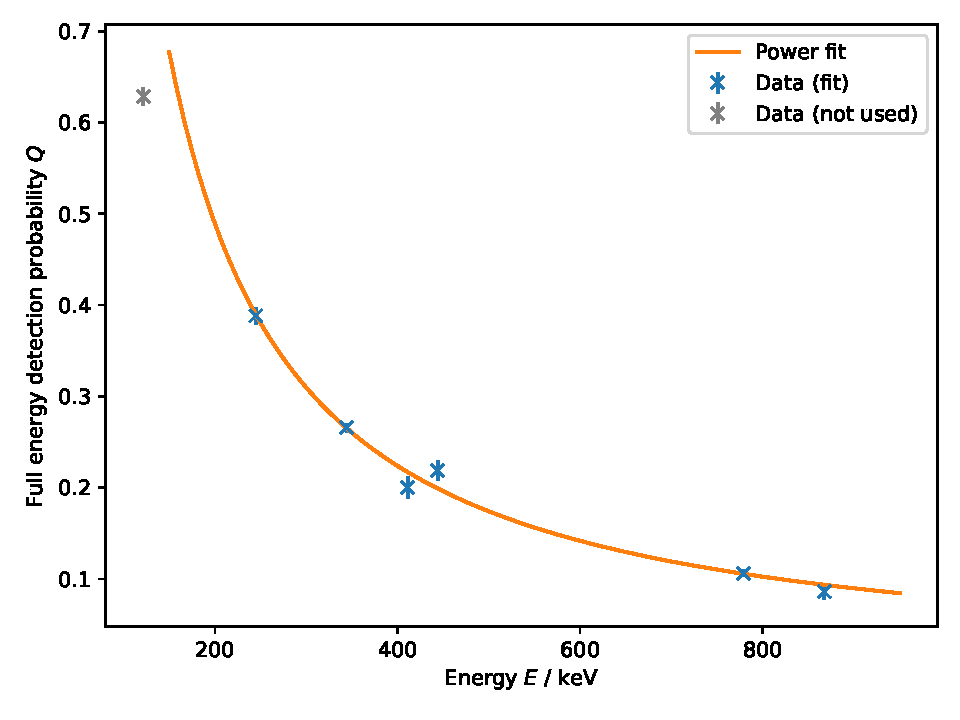
\includegraphics[width=0.8\textwidth]{content/plots/eu_efficiency.pdf}
    \caption{Full energy detection probability $Q$ in dependence of the energy with a power fit for $E > \SI{150}{keV}$.}
    \label{fig:eu_efficiency}
\end{figure}

\begin{table}[H]
	\centering
	\caption{Line contents $N$ and full energy detection probabilities $Q$ of the \ce{^{152}Eu} lines.}
	\label{tab:eu_Q}
	\begin{tabular}{c  c  c}
		\toprule
		$E_\gamma$ / keV & $N$ / s$^{-1}$ & $Q$\\
		\midrule
		121.78 & 5.884  \, \clap{$\pm$} \,  0.035 & 0.3910  \, \clap{$\pm$} \,  0.0063 \\
		 244.70 & 0.964  \, \clap{$\pm$} \,  0.020 & 0.2416  \, \clap{$\pm$} \,  0.0061 \\
		 344.28 & 2.305  \, \clap{$\pm$} \,  0.023 & 0.1652  \, \clap{$\pm$} \,  0.0047 \\
		 411.12 & 0.1462  \, \clap{$\pm$} \,  0.0087 & 0.1243  \, \clap{$\pm$} \,  0.0077 \\
		 443.96 & 0.2020  \, \clap{$\pm$} \,  0.0099 & 0.1219  \, \clap{$\pm$} \,  0.0063 \\
		 778.90 & 0.450  \, \clap{$\pm$} \,  0.016 & 0.0661  \, \clap{$\pm$} \,  0.0027 \\
		 867.37 & 0.119  \, \clap{$\pm$} \,  0.011 & 0.0534  \, \clap{$\pm$} \,  0.0051 \\
		 \bottomrule
	\end{tabular}
\end{table}


\subsection{Monochromatic gamma source \texorpdfstring{\ce{^{137}Cs}}{137Cs}}

For the monochromatic gamma source the measurements are shown in \autoref{fig:monochromatic_Cs}, where the background is subtracted from the measured data per second.
This measurement was taken for 1 hour 18 minutes and 57 seconds.
The channels were converted to energies with \autoref{eqn:lin}.
In the plot the compton continuum can be seen up to the orange vertical line, and the backscatter peak is shown by the green line. In addition to that the photopeak is clearly
visible at an energy around $\SI{661}{keV}$.


\begin{figure}[htbp]
    \centering
    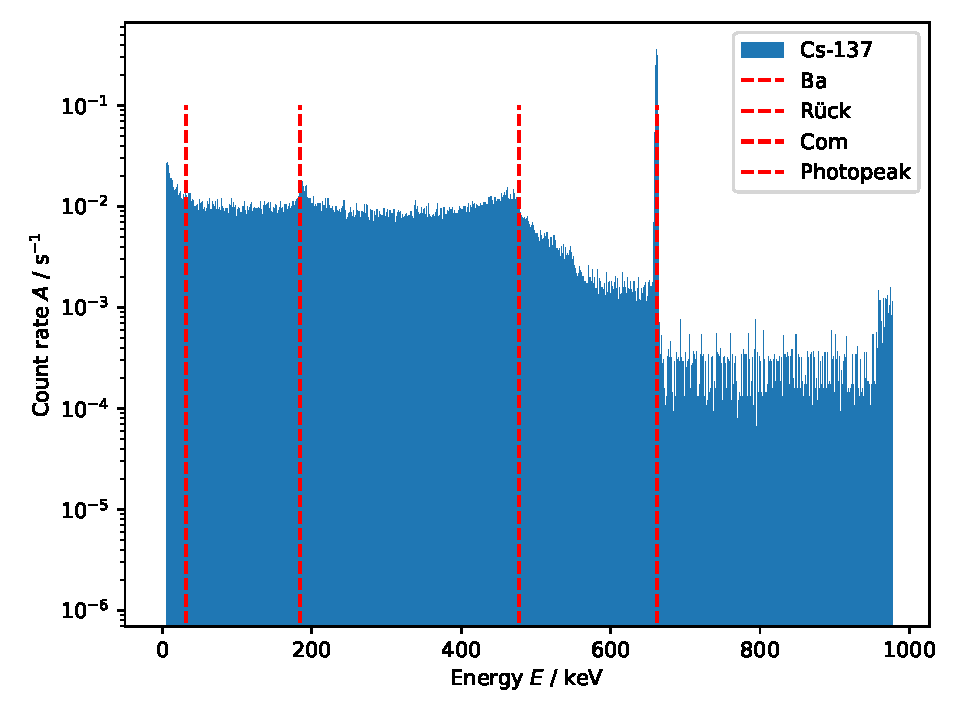
\includegraphics[width=0.8\textwidth]{content/plots/monochromatic_Cs.pdf}
    \caption{Measured spectrum of \ce{^{137}Cs} with the positions of the backscatter peak, the Compton edge and the photopeak.}
    \label{fig:monochromatic_Cs}
\end{figure}

40 channels around the photopeak are shown in \autoref{fig:photopeak_Cs}. In it also a gaussian fit is seen with the full width at half maximum and the full width at tenth maximum.
The gaussian fit is done the same way as for the \ce{^{152}Eu} lines with \autoref{eqn:gauss} and gives the position of the photopeak
\begin{equation}
    E_\text{photo} = \SI{661.6 \pm 0.4}{keV} \ .
\end{equation}
% which fits very well to the literature value of $\SI{661.657}{keV}$.
The width of the peak is $\sigma = \SI{1.013 \pm 0.008}{keV}$.
From this the full width at half maximum and the full width at tenth maximum are calculated through
\begin{align}
    \text{FWHM} &= 2\sqrt{2\ln 2} \cdot \sigma \\
    \text{FWTM} &= 2\sqrt{2\ln 10} \cdot \sigma \ .
\end{align}
The results are
\begin{align}
    \text{FWHM} &= \SI{2.386 \pm 0.020}{keV} \\
    \text{FWTM} &= \SI{4.35 \pm 0.04}{keV} \ .
\end{align}
The line content of the photopeak is calculated like before with $N = \sqrt{2\pi}\cdot h \cdot \sigma$, which gives
\begin{equation}
    N_\text{photo} = \SI{7.39 \pm 0.07}{\per\second} \ .
\end{equation}

\begin{figure}[htbp]
    \centering
    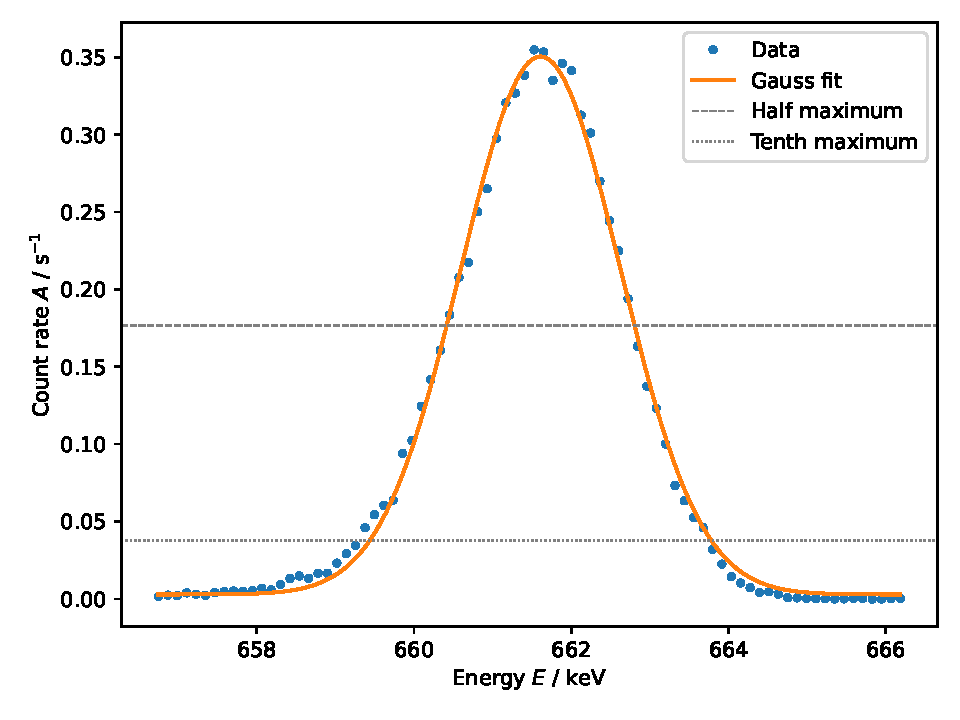
\includegraphics[width=0.8\textwidth]{content/plots/photopeak_Cs.pdf}
    \caption{Gaussian fit of the photopeak of \ce{^{137}Cs} with the full width at half and at tenth maximum.}
    \label{fig:photopeak_Cs}
\end{figure}

\subsubsection*{Compton edge and backscatter peak}

The backscatter peak is again found through scipy and then a range of 200 channels is plotted and fitted with a gaussian.
This plot is seen in \autoref{fig:backscatter_Cs}.
The peak is measured at $E = \SI{188.9\pm 0.4}{keV}$.
The compton edge is measured at $E_{ce}= \SI{477}{keV}$.


\begin{figure}[htbp]
    \centering
    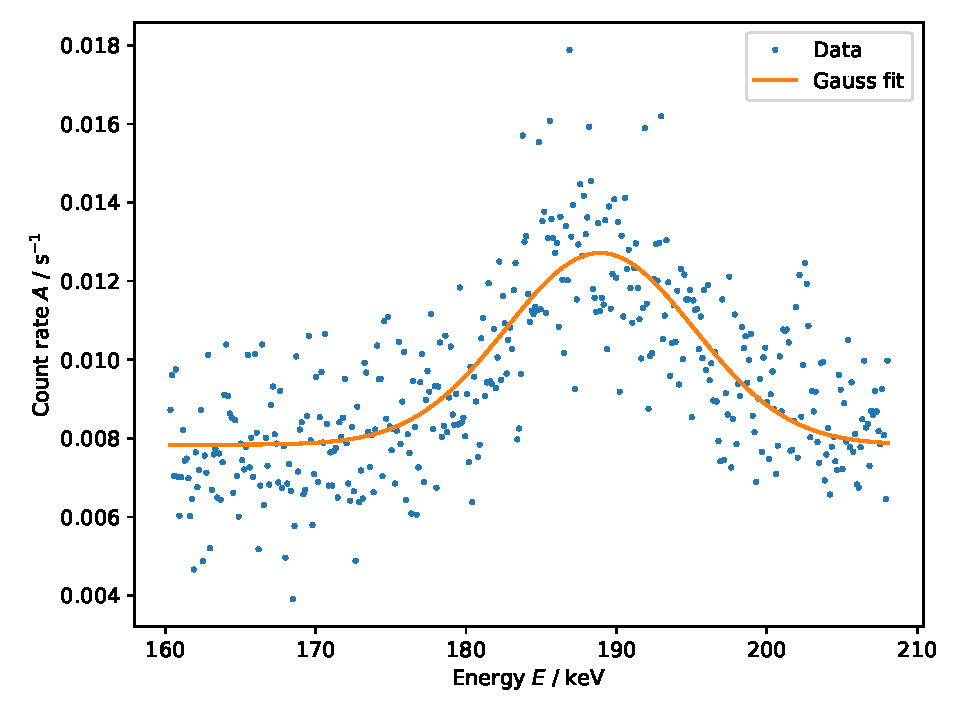
\includegraphics[width=0.8\textwidth]{content/plots/backscatter_Cs.pdf}
    \caption{Gaussian fit of the backscatter peak of \ce{^{137}Cs}.}
    \label{fig:backscatter_Cs}
\end{figure}

\subsubsection*{Compton continuum}

The compton continuum is described by the Klein-Nishina formula \eqref{eq:klein_nishina}.
Written in dependence of the energy $T$ of the scattered electron, it gives the fit function
\begin{equation}
    \frac{\text d \sigma}{\text d T} = A_c \left(2 + \frac{s^2}{\varepsilon^2(1-s)^2} + \frac{s}{1-s}\left(s - \frac{2}{\varepsilon}\right)\right) \ ,
    \label{eqn:compton_fit}
\end{equation}
with $s = T/E_\gamma$ and $\varepsilon = E_\gamma / (m_e c^2)$.
Here $T$ is the energy of the electron, $E_\gamma = \SI{661.657}{keV}$ the energy of the gamma ray and $A_c$ the only fit parameter.
The fit is done in the range from $\SI{350}{keV}$ to $\SI{460}{keV}$, because there the continuum is not disturbed by the backscatter peak and is still below the compton edge.
The fit and the measured data are shown in \autoref{fig:compton_Cs}.
The fit gives the parameter
\begin{equation}
    A_c = \num{3.606 \pm 0.021 e-3} \ .
\end{equation}
The line content of the compton continuum is calculated by summing up the fit function over all channels from $\SI{0}{keV}$ to the compton edge, which gives
\begin{equation}
    N_\text{compton} = \SI{26.55 \pm 0.15}{\per\second} \ .
\end{equation}
So the ratio between the line content of the photopeak and the compton continuum is
\begin{equation}
    \frac{N_\text{photo}}{N_\text{compton}} = \num{0.2784 \pm 0.0030} \ .
\end{equation}
\\
This is compared with the absorption probability $P$ of the gamma rays in the detector from \eqref{eq:absorption}, with the length of the germanium crystal $z = l = \SI{3.9}{cm}$.
The extinction coefficients for $\SI{662}{keV}$ are read from \autoref{fig:exctinct} with $\mu_\text{photo} = \SI{0.008}{\per\centi\meter}$ and $\mu_\text{compton} = \SI{0.37}{\per\centi\meter}$.
This gives
\begin{align}
    P_\text{photo} &= \num{0.031} \\
    P_\text{compton} &= \num{0.764} \ ,
\end{align}
so the ratio is $P_\text{photo}/P_\text{compton} = \num{0.040}$.



\begin{figure}[htbp]
    \centering
    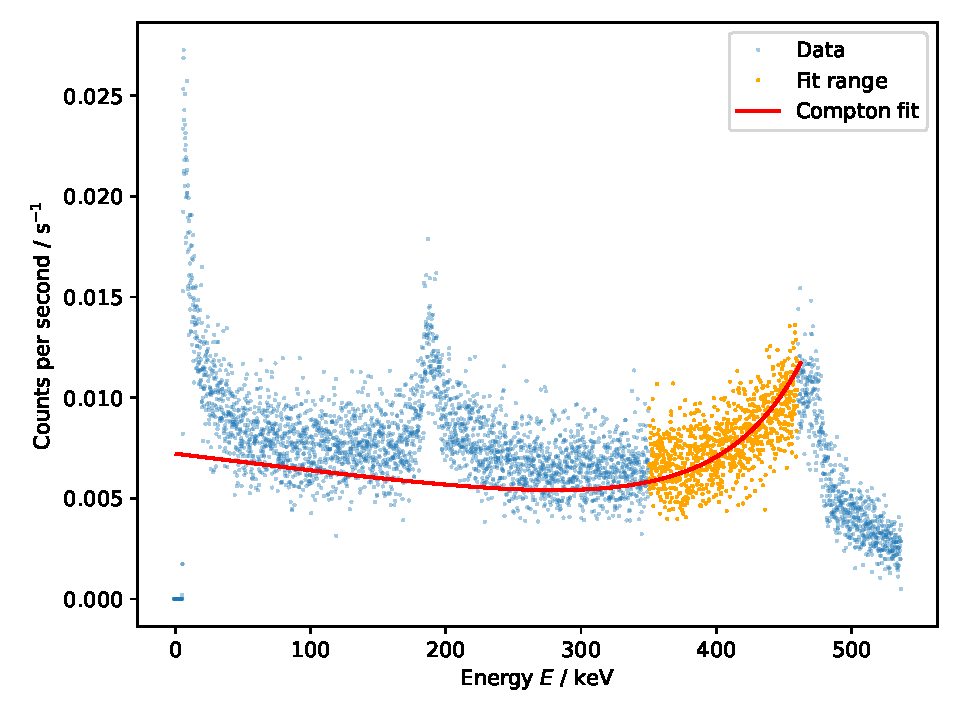
\includegraphics[width=0.8\textwidth]{content/plots/compton_Cs.pdf}
    \caption{Compton continuum of \ce{^{137}Cs} with the fit of the differential cross section.}
    \label{fig:compton_Cs}
\end{figure}

\subsection{Activity determination of \texorpdfstring{\ce{^{133}Ba}}{133Ba}}

The data of the measurement of \ce{^{133}Ba} for a time of 1 hour 4 minutes and 6 seconds are shown as a rate per second in \autoref{fig:barium}.
In this plot the peaks are again found with scipy. These peaks are listed in \autoref{tab:ba_activity}.
Here also only peaks above $\SI{150}{keV}$ are used, because the Q fit is only usable for energies $>\SI{150}{keV}$.


\begin{figure}[htbp]
    \centering
    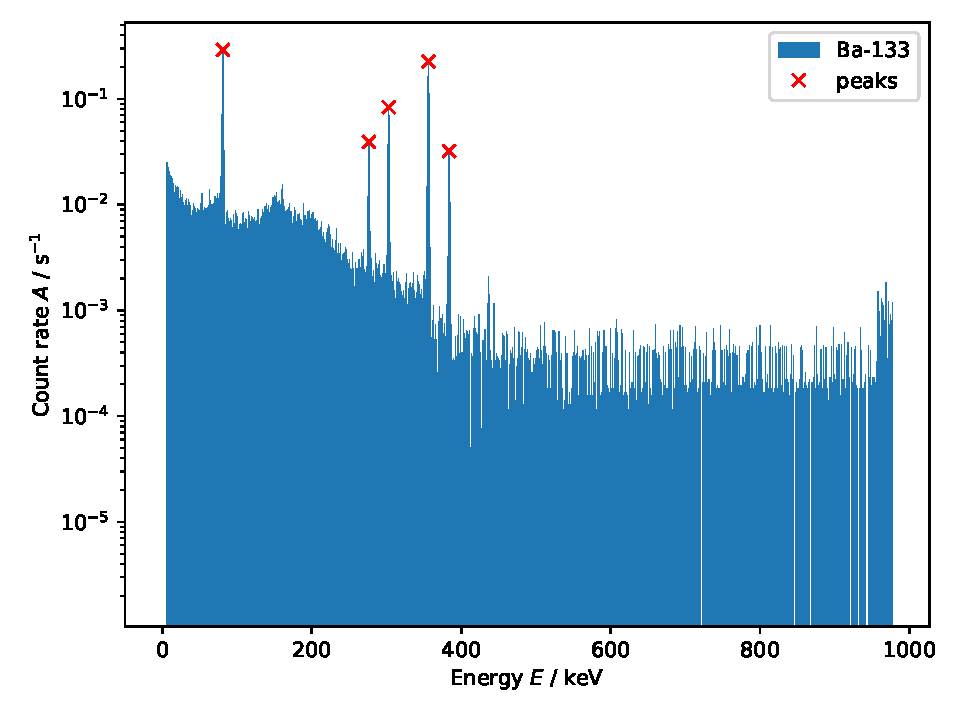
\includegraphics[width=0.8\textwidth]{content/plots/barium.pdf}
    \caption{Measured spectrum of \ce{^{133}Ba} with the found peaks.}
    \label{fig:barium}
\end{figure}

The line contents are again determined like before with a plot like \autoref{fig:barium_gauss_fit} and a gaussian fit.
With this the values shown in \autoref{tab:ba_activity} are calculated.

\begin{figure}[htbp]
    \centering
    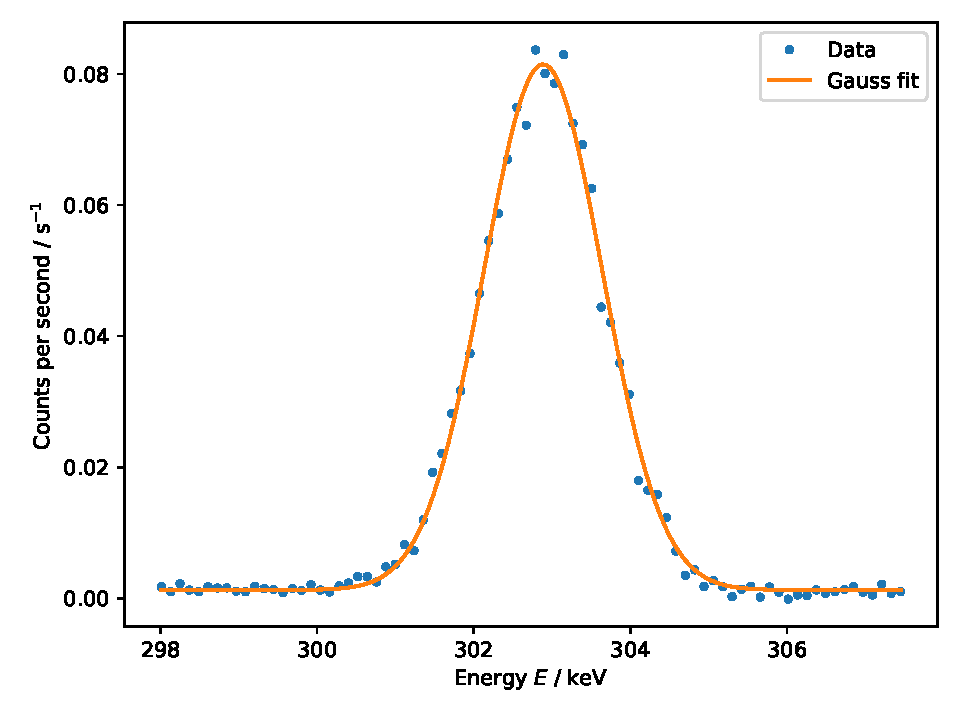
\includegraphics[width=0.8\textwidth]{content/plots/barium_gauss_fit.pdf}
    \caption{Gaussian fit of the $\SI{302.9}{keV}$ line of \ce{^{133}Ba} as an example for the determination of the line content.}
    \label{fig:barium_gauss_fit}
\end{figure}

\subsubsection*{Activity}

To calculate the activity, \autoref{eqn:Q} is rearranged for $A$ and the probability is taken from \autoref{tab:ba_lit}.
With this the activities shown in \autoref{tab:ba_activity} are calculated.
A new solid angle is used, because $a$ is changed to $a = \SI{7.9}{cm}-\SI{4.665}{cm}+\SI{1.5}{cm}$.
The mean value of the activity results in $A = \SI{771\pm 10}{Bq}$.

\begin{table}[H]
	\centering
	\caption{Energies $E_\gamma$ and emission probabilities $W$ of the used \ce{^{133}Ba} gamma lines~\cite{ba133}.}
	\label{tab:ba_lit}
	\begin{tabular}{c  c}
		\toprule
		$E_\gamma$ / keV & $W$ / \%\\
		\midrule
		276.40 & 7.164  \, \clap{$\pm$} \,  0.022 \\
		 302.85 & 18.330  \, \clap{$\pm$} \,  0.060 \\
		 356.02 & 62.05  \, \clap{$\pm$} \,  0.19 \\
		 383.85 & 8.940  \, \clap{$\pm$} \,  0.030 \\
		 \bottomrule
	\end{tabular}
\end{table}


\begin{table}[H]
	\centering
	\caption{Fitted energies $E$, line contents $N$, full energy detection probabilities $Q$ and activities $A$ of the \ce{^{133}Ba} lines.}
	\label{tab:ba_activity}
	\begin{tabular}{c  c  c  c}
		\toprule
		$E$ / keV & $N$ / s$^{-1}$ & $Q$ & $A$ / Bq\\
		\midrule
		276.41  \, \clap{$\pm$} \,  0.26 & 0.577  \, \clap{$\pm$} \,  0.010 & 0.2099  \, \clap{$\pm$} \,  0.0039 & 792  \, \clap{$\pm$} \,  21 \\
		 302.89  \, \clap{$\pm$} \,  0.26 & 1.274  \, \clap{$\pm$} \,  0.014 & 0.1891  \, \clap{$\pm$} \,  0.0032 & 759  \, \clap{$\pm$} \,  16 \\
		 356.05  \, \clap{$\pm$} \,  0.28 & 3.541  \, \clap{$\pm$} \,  0.025 & 0.1573  \, \clap{$\pm$} \,  0.0025 & 750  \, \clap{$\pm$} \,  13 \\
		 383.85  \, \clap{$\pm$} \,  0.28 & 0.4879  \, \clap{$\pm$} \,  0.0094 & 0.1444  \, \clap{$\pm$} \,  0.0023 & 781  \, \clap{$\pm$} \,  20 \\
		 \bottomrule
	\end{tabular}
\end{table}


\subsection{Gamma spectrum of an unknown source}

The data of the unknown source were measured for 1 hour 2 minutes and 15 seconds and are shown as a rate per second in \autoref{fig:unknown}.
The peaks are again found with scipy and only peaks above $\SI{150}{keV}$ are used, like before.
For every peak a gaussian fit with \autoref{eqn:gauss} is done, which gives the energies and line contents shown in \autoref{tab:unknown_lines}.
\\
To identify the source, these energies are compared with the database of the NNDC~\cite{nndc}.
The peak at $\SI{186}{keV}$ belongs to \ce{^{226}Ra}, the peaks at $\SI{242}{keV}$, $\SI{295}{keV}$ and $\SI{352}{keV}$ to \ce{^{214}Pb}
and the peak at $\SI{609}{keV}$ to \ce{^{214}Bi}.
All of them are part of the decay chain of \ce{^{238}U}, where \ce{^{214}Pb} and \ce{^{214}Bi} are daughter nuclides of \ce{^{226}Ra}.
The peak at $\SI{186}{keV}$ could also be from \ce{^{235}U} with an energy of $\SI{185.72}{keV}$, which cannot be distinguished here.

\begin{figure}[htbp]
    \centering
    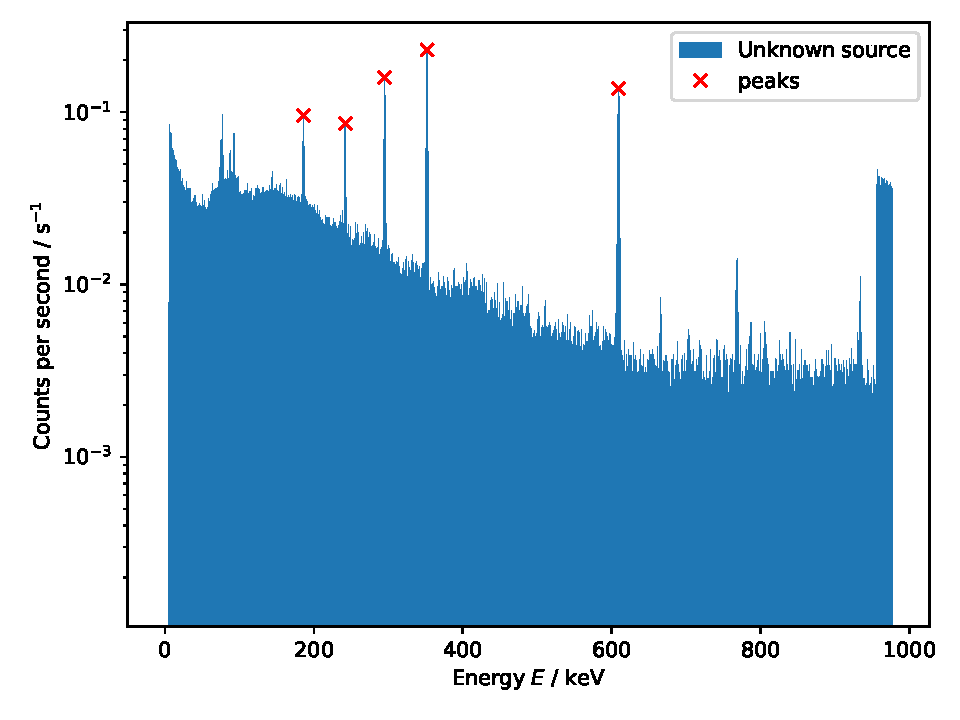
\includegraphics[width=0.8\textwidth]{content/plots/unknown.pdf}
    \caption{Measured spectrum of the unknown source with the found peaks.}
    \label{fig:unknown}
\end{figure}

\begin{table}[H]
	\centering
	\caption{Fitted energies $E$ and line contents $N$ of the unknown source with the assigned nuclides and their literature energies $E_\text{lit}$ and emission probabilities $W$~\cite{nndc}.}
	\label{tab:unknown_lines}
	\begin{tabular}{c  c  c  c  c}
		\toprule
		$E$ / keV & $N$ / s$^{-1}$ & Nuclide & $E_\text{lit}$ / keV & $W$ / \%\\
		\midrule
		185.96  \, \clap{$\pm$} \,  0.24 & 1.019  \, \clap{$\pm$} \,  0.025 & \ce{^{226}Ra} & 186.21 & 3.64 \\
		 242.00  \, \clap{$\pm$} \,  0.25 & 0.983  \, \clap{$\pm$} \,  0.022 & \ce{^{214}Pb} & 242.00 & 7.27 \\
		 295.21  \, \clap{$\pm$} \,  0.26 & 2.112  \, \clap{$\pm$} \,  0.026 & \ce{^{214}Pb} & 295.22 & 18.41 \\
		 351.91  \, \clap{$\pm$} \,  0.28 & 3.529  \, \clap{$\pm$} \,  0.033 & \ce{^{214}Pb} & 351.93 & 35.60 \\
		 609.31  \, \clap{$\pm$} \,  0.35 & 2.622  \, \clap{$\pm$} \,  0.038 & \ce{^{214}Bi} & 609.32 & 45.49 \\
		 \bottomrule
	\end{tabular}
\end{table}


\subsubsection*{Activity}

The activities are calculated the same way as for \ce{^{133}Ba} with \autoref{eqn:Q} and the same solid angle. The results are shown in \autoref{tab:unknown_activity}.
For \ce{^{214}Pb} the mean value of the three lines is taken.
This gives the activities
\begin{align}
    A_{\ce{^{226}Ra}} &= \SI{1750 \pm 70}{Bq} \\
    A_{\ce{^{214}Pb}} &= \SI{1216 \pm 41}{Bq} \\
    A_{\ce{^{214}Bi}} &= \SI{1400 \pm 40}{Bq} \ .
\end{align}

\begin{table}[H]
	\centering
	\caption{Full energy detection probabilities $Q$ and activities $A$ of the lines of the unknown source.}
	\label{tab:unknown_activity}
	\begin{tabular}{c  c  c  c}
		\toprule
		Nuclide & $E_\text{lit}$ / keV & $Q$ & $A$ / Bq\\
		\midrule
		\ce{^{226}Ra} & 186.21 & 0.3298  \, \clap{$\pm$} \,  0.0098 & 1753  \, \clap{$\pm$} \,  68 \\
		 \ce{^{214}Pb} & 242.00 & 0.2443  \, \clap{$\pm$} \,  0.0053 & 1144  \, \clap{$\pm$} \,  36 \\
		 \ce{^{214}Pb} & 295.22 & 0.1948  \, \clap{$\pm$} \,  0.0034 & 1217  \, \clap{$\pm$} \,  26 \\
		 \ce{^{214}Pb} & 351.93 & 0.1594  \, \clap{$\pm$} \,  0.0025 & 1285  \, \clap{$\pm$} \,  23 \\
		 \ce{^{214}Bi} & 609.32 & 0.0853  \, \clap{$\pm$} \,  0.0021 & 1397  \, \clap{$\pm$} \,  40 \\
		 \bottomrule
	\end{tabular}
\end{table}


\clearpage
